\subsection{IU Realizar pago de cita}

\subsubsection{Objetivo}
Registrar el pago de una cita para que el paciente pueda acceder a ésta.

\subsubsection{Diseño}
Esta pantalla aparece al hacer click sobre "Realizar pago de cita" al haber iniciado sesión como cajero.

\begin{figure}[htbp!]
	\centering
	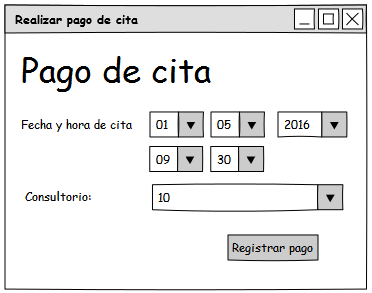
\includegraphics[width=0.8\textwidth]{images/IU_pagar_cita}
	\caption{IU Realizar pago de cita}
\end{figure}


\subsubsection{Salidas}
\begin{itemize} 
	\item Mensaje de confirmación: Cadena "Pago registrado correctamente"
	\item Información de cita:
	\begin{itemize}
		\item Fecha de cita: Fecha en formato dd/mm/yyyy
		\item Hora de cita: Hora con formato hh:mm
		\item Consultorio de cita: Número entero entre 1 y 12
	\end{itemize}
\end{itemize}
\subsubsection{Entradas}
\begin{itemize}
	\item ID de la cita: entero positivo
\end{itemize}

\subsubsection{Comandos}
\begin{itemize}
	\item \IUbutton{Registrar pago}:  Verifica que el la cita exista, tenga fecha y hora posterior a las actuales y haya sido pagada. En tal caso, se actualiza el estado de la cita a pagada.  \IUref{UI2}{Home}.	
\end{itemize}

\subsubsection{Mensajes}
\begin{Citemize}
	\item {\bf MSGb} Cita no existe
	\item {\bf MSGc} La cita expiró
	\item {\bf MSGd} Cita ya está pagada
	\item {\bf MSGe} Complete todos los campos
	\item {\bf MSGf} Formato de campos inválido
\end{Citemize}

\subsection{IU Crear expediente}

\subsubsection{Objetivo}
Registrar los datos y antecedentes médicos de un paciente.

\subsubsection{Diseño}
Esta pantalla aparece al hacer click sobre "Atender paciente" y es la primera consulta del paciente, al haber iniciado sesión como médico.

\begin{figure}[htbp!]
	\centering
	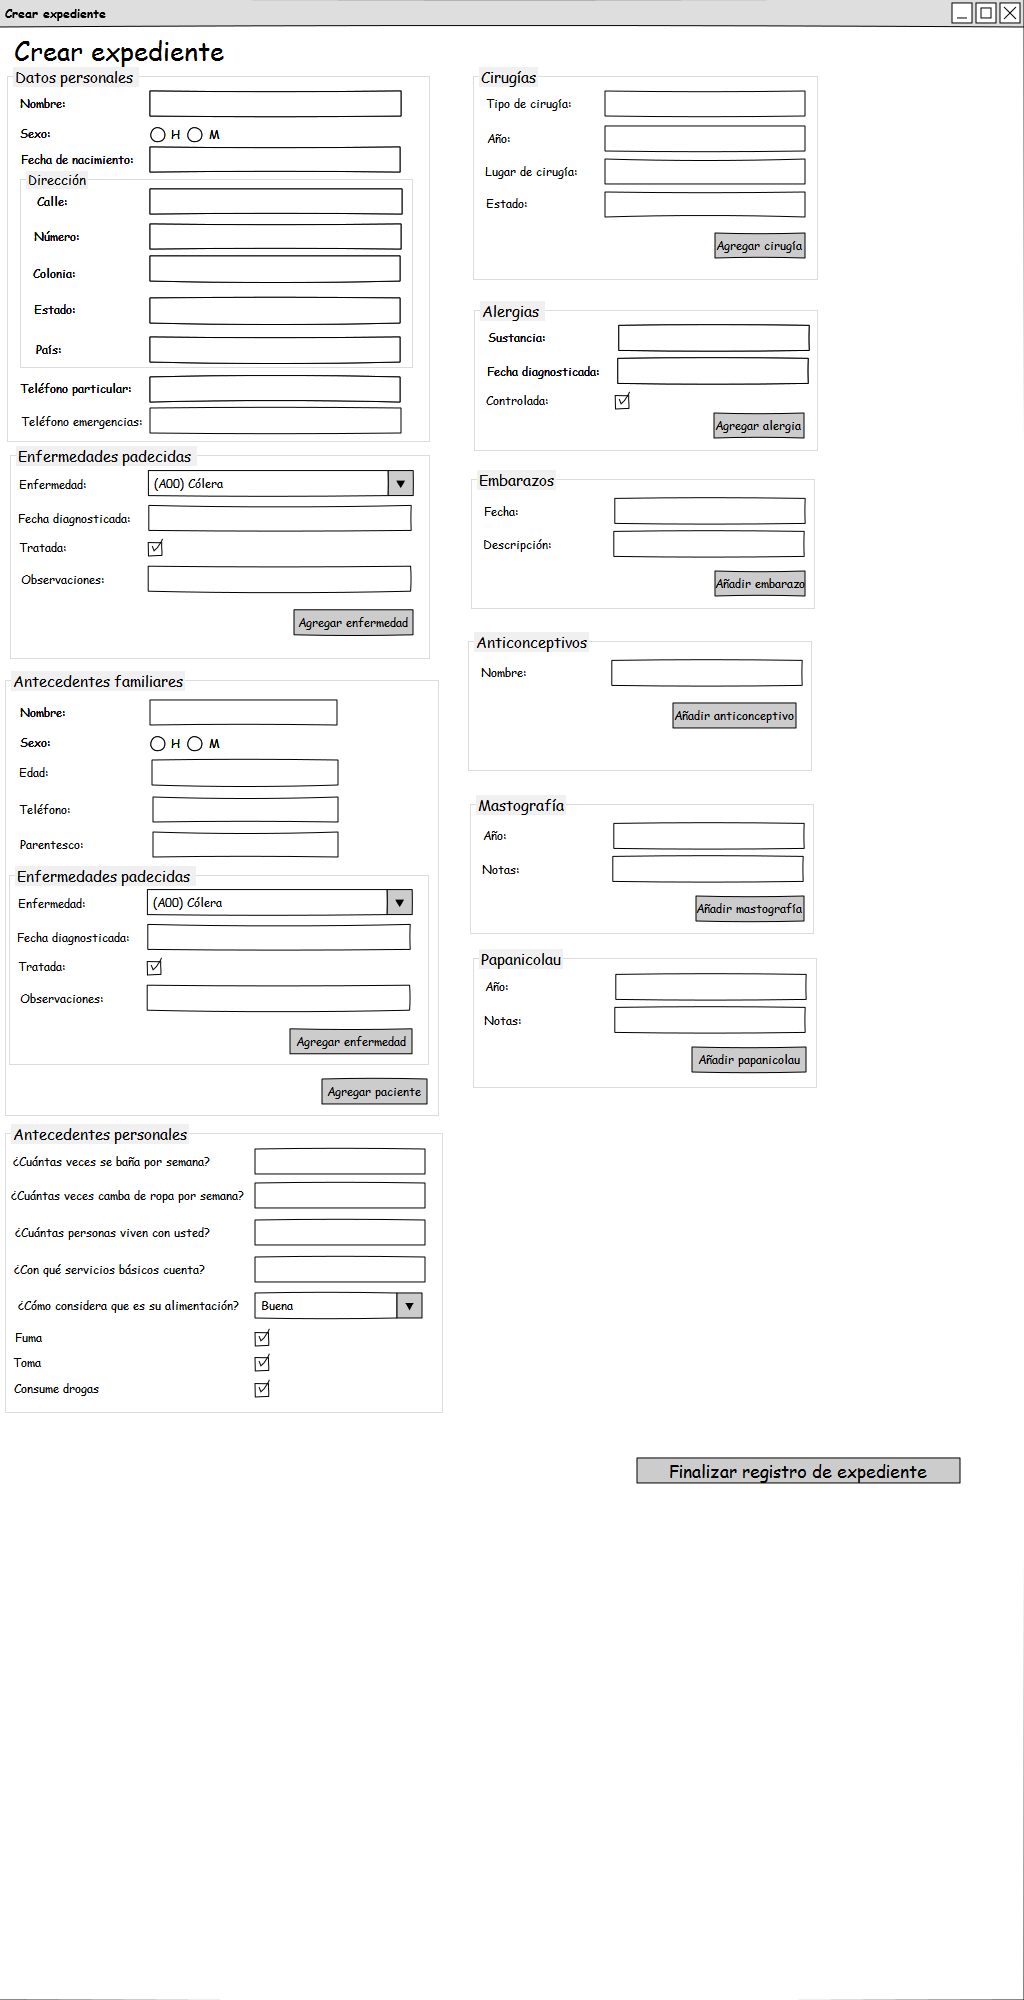
\includegraphics[width=0.8\textwidth]{images/IU_crear_expediente}
	\caption{IU Crear expediente}
\end{figure}


\subsubsection{Salidas}
\begin{itemize} 
	\item Listadas en el caso de uso CU6 "Crear expediente"
\end{itemize}
\subsubsection{Entradas}
\begin{itemize}
	\item Listadas en el caso de uso CU6 "Crear expediente"
\end{itemize}

\subsubsection{Comandos}
\begin{itemize}
	\item \IUbutton{Finalizar registro de expediente}:  Verifica que hayan sido ingresados los datos requeridos y tengan formato correcto, de ser así, se guardan datos del expediente y se notifica al médico.  \IUref{UI2}{Home}.	
	\item \IUbutton{Agregar enfermedad}:  Agrega un elemento a la lista de enfermedades del paciente o de un familiar .
	\item \IUbutton{Agregar familiar}:  Agrega un elemento a la lista de antecedentes familiares del paciente .
	\item \IUbutton{Agregar cirugía}:  Agrega un elemento a la lista de cirugías del paciente .
	\item \IUbutton{Agregar alergia}:  Agrega un elemento a la lista de alergias del paciente .
	\item \IUbutton{Agregar embarazo}:  Agrega un elemento a la lista de embarazos del paciente .
	\item \IUbutton{Agregar anticonceptivo}:  Agrega un elemento a la lista de anticonceptivos del paciente .
	\item \IUbutton{Agregar mastografía}:  Agrega un elemento a la lista de mastografías del paciente .
	\item \IUbutton{Agregar papanicolau}:  Agrega un elemento a la lista de papanicolaus del paciente .
\end{itemize}

\subsubsection{Mensajes}
\begin{Citemize}
	\item {\bf MSGa} Expediente creado correctamente
	\item {\bf MSGb} Complete todos los campos
	\item {\bf MSGc} Formato de campos inválido
\end{Citemize}

